%!TEX root = ../report.tex


\chapter{Software Requirements Specification (SRS)}\label{ch:software-requirements-specification-(srs)}


\section{Introduction}\label{sec:introduction}
The first section of the document will describe the scope of the project as well as provide an overview of the items
contained in this SRS document.
In addition to this it will provide a purpose to this document as well as a list of abbreviations.

\subsection{Purpose}\label{subsec:purpose}
This document has been developed to build a fully encrypted chat application called SocialStuff or as of now Trale with
localized data storage and to provide you, as the lecturer, with an overview of this project.
The requirements for the Trale application have been derived from the provided pdf file on Sharepoint as well as
interviews and personal meetings with J\"orn Neumeyer who came up with the project and was in close contact with Gedak
GmbH who submitted the project for the software factory.
This document has been developed to allow you, as the lecturer, to get an understanding of the requirements for an
elevator API specification.

\subsection{Scope of project}\label{subsec:scope-of-project}
The product is a chat application, which is intended to offer an open, decentralized alternative to current proprietary
and centralized communication and social media platforms.
The decentralized model allows for an independent utilization of the software, providing companies as well as normal
users with more sovereignty and less dependence on large service providers.
Some parts of the system are already provided but might need to be extended upon for further functionality.

The development will be split in frontend and backend development.
The following part of the SRS will specify the scope for each of the components which are to be developed, to achieve
the overarching goal of a functioning application.

\subsubsection{Backend Scope}
\begin{itemize}
    \item \textbf{Identity Service}
    The identity service will handle the identity management for the users and handle the permissions each of the users
    will have.
    \item \textbf{File Service}
    The file service will handle the forwarding of the files which can be sent via the chat application.
    \item \textbf{Reporting Service}
    The reporting service will handle the reporting mechanic of the chat application.
    The application will be able to allow the reporting of users.
    The service will be able to handle administrative tasks, such as adding reasons which users can be reported for,
    (un)blocking users and the reporting itself.
    \item \textbf{Settings Service}
    The Settings service provides an interface to the admin panel frontend and carries out the settings to the other
    services (e.g.\ reporting settings will be affecting the reporting service, creating invite codes to a server will
    affect the identity service).
    \item
\end{itemize}

\subsubsection{Frontend Scope}
% TODO add scope of frontend

\begin{enumerate}
    \item Admin
    The Admin Panel offers the administrators of the application many setting options.
    When an admin logs in, he or she is redirected directly to the Admin Panel.
    \begin{enumerate}
        \item Dashboard
        The Dashboard gives the administrators an overview of the Data which is saved on the server.
        Due to the aim of this project to protect the user’s privacy, the data depth will be limited.
        \item Security settings
        This Component gives the opportunity, to change the security settings of the chat application.
        The way of authentication and the format of the password can be decided.
        It will also be possible to set an option for only letting users with an invite code onto the server.
        \item Create invites
        This Component shows a list of all invite codes existing on the server and the possibility to delete them.
        It is also possible to add a new invite code with all attributes needed for it.
        An invite code could also be generated.
        \item Report Settings
        On this component the administrators can create report reasons which can be used by the application’s users
        to report their chat partners.
        The report reasons created can be changed or deleted.
        All reasons are shown in a list.
        In addition, it can be set if the system should automatically block users.
        \item Reported Users
        The Reported Users component shows a list of all users which have been reported by other users.
        The list will also show the reasons including the times the user was reported because of it.
        The times a user was reported for each reason are added up, showing a total number of reports.
        \item Banned Users
        This Component will show all users which where banned from the web service.
        Like the Reported Users component, described in 1.6, the reasons and the total number of reports are shown.
        The administrators have the possibility to unban a user, giving him or her back access to the site.
    \end{enumerate}
\end{enumerate}

\subsection{Definitions}\label{subsec:definitions}

\begin{table}[ht]
    \begin{tabular}{|l|l|}
        \toprule
        \textbf{Term} & \textbf{Definition}                                                          \\
        \midrule
        SRS           & Software Requirements Specification                                          \\
        \midrule
        Must &
        \begin{tabular}[c]{@{}l@{}}
            This word, or the terms "REQUIRED" or "SHALL", mean that the definition is an\\  absolute requirement of the specification.
        \end{tabular} \\
        \midrule
        Will          & Must be implemented, cannot be verified.                                     \\
        \midrule
        Should &
        \begin{tabular}[c]{@{}l@{}}
            This word, or the adjective "RECOMMENDED", mean that there \\ may exist valid reasons in particular circumstances to ignore\\ a particular item, but the full implications must be understood \\ and carefully weighed before choosing a different course.
        \end{tabular} \\
        \midrule
        Stakeholder & A stakeholder is a party with an interest in an enterprise or project. \\
        \midrule
        Administrator & \begin{tabular}[c]{@{}l@{}}
                            The user which has access to settings related to the functioning of the chat\\ application.
        \end{tabular} \\
        \midrule
        Invite Code & \begin{tabular}[c]{@{}l@{}}
                          A set of characters giving a new user the possibility to register to the web\\ service.
        \end{tabular} \\
        \midrule
        Report Reason & A reason any user can choose for another user, blaming one for bad behavior. \\
        \midrule
        Reported User & A user for which a report reason has been chosen by a chat partner. \\
        \midrule
        Banned User & \begin{tabular}[c]{@{}l@{}}
                          A user which who was taken away of the ability to login to the chat\\ application.
        \end{tabular} \\
        \midrule
        Admin Panel & \begin{tabular}[c]{@{}l@{}}
                          Part of the web application where administrators can change the settings\\ of the server.
        \end{tabular} \\
        \bottomrule
    \end{tabular}
    \label{tab:table24}
\end{table}

\subsection{Overview of Document}\label{subsec:overview-of-document}
The next chapter of this document gives an overview of the functionality of the product.
It describes the informal requirements and is used to establish a context for the technical requirements specification.
In the next chapter different stakeholders will be introduced.
The third chapter, requirements specification section, of this document is written primarily for the developers and
describes in technical terms the details of the functionality of the product.


\section{Overall Description}\label{sec:overall-description}
This section will give a general overview of the whole system and the main stakeholders of the elevator API
specification.

\subsection{Product Perspective}\label{subsec:product-perspective}
The Application is a chat application that requires user interaction.
This means the application will contain a frontend, that is easy to understand for the end user and does not require a
huge amount of technical knowledge.
The main encryption and decryption will take place automatically without the user even noticing that such a thing
exists in the background.
To make future development easier, the project will also include a proper documentation of the parts of the software
that were developed in this semester.

The following main features will exist in the end of the project:
\begin{itemize}
    \setlength\itemsep{-0.5em}
    \item A user-friendly user interface
    \item A backend that prevents tracing of messages and provides the necessary features for the frontend
    \item An administrator interface that allows configurating the server
    \item A documentation of everything that has been created this semester.
\end{itemize}

\subsection{Product Functions}\label{subsec:product-functions}
With the chat application, users will be certain, that the information they share will only be readable by the intended
receiver, no third party will be able to access the information.
The user however should still have the maximum amount of comfort possible, while using the application to prevent him
from going back to existing, non-encrypted chat services for comfort reasons.
Setting up the server of the application might require some basic IT-knowledge, but it shouldn’t be too excessive
(No programming knowledge, but proper software setup knowledge).
The result of using the system is that the sharing of information sharing will become more secure and less transparent,
whilst keeping user comfort at a maximum.

\subsection{User Characteristics}\label{subsec:user-characteristics}

There are two types of users using the system:

\paragraph{Regular User}
The regular user is a normal person. They use the system as a normal chat application without having to think about the
complicated processes happening in the background.
They will just use the main frontend.

\paragraph{Administrator}
The Administrator sets up the server.
He requires some basic IT knowledge.
He will setup the server and use the Admin panel which can be used to conduct configurations.

~\ref{fig:figure5} shows the use case diagram for the admin panel.
It also separates the system into the different backend services, therewith showing the responsibility for each use
case.
As can be derived from this diagram, the admin can conduct administrative tasks whilst the user can only conduct tasks
that are end user related.

\begin{figure}[h]
    \centering
    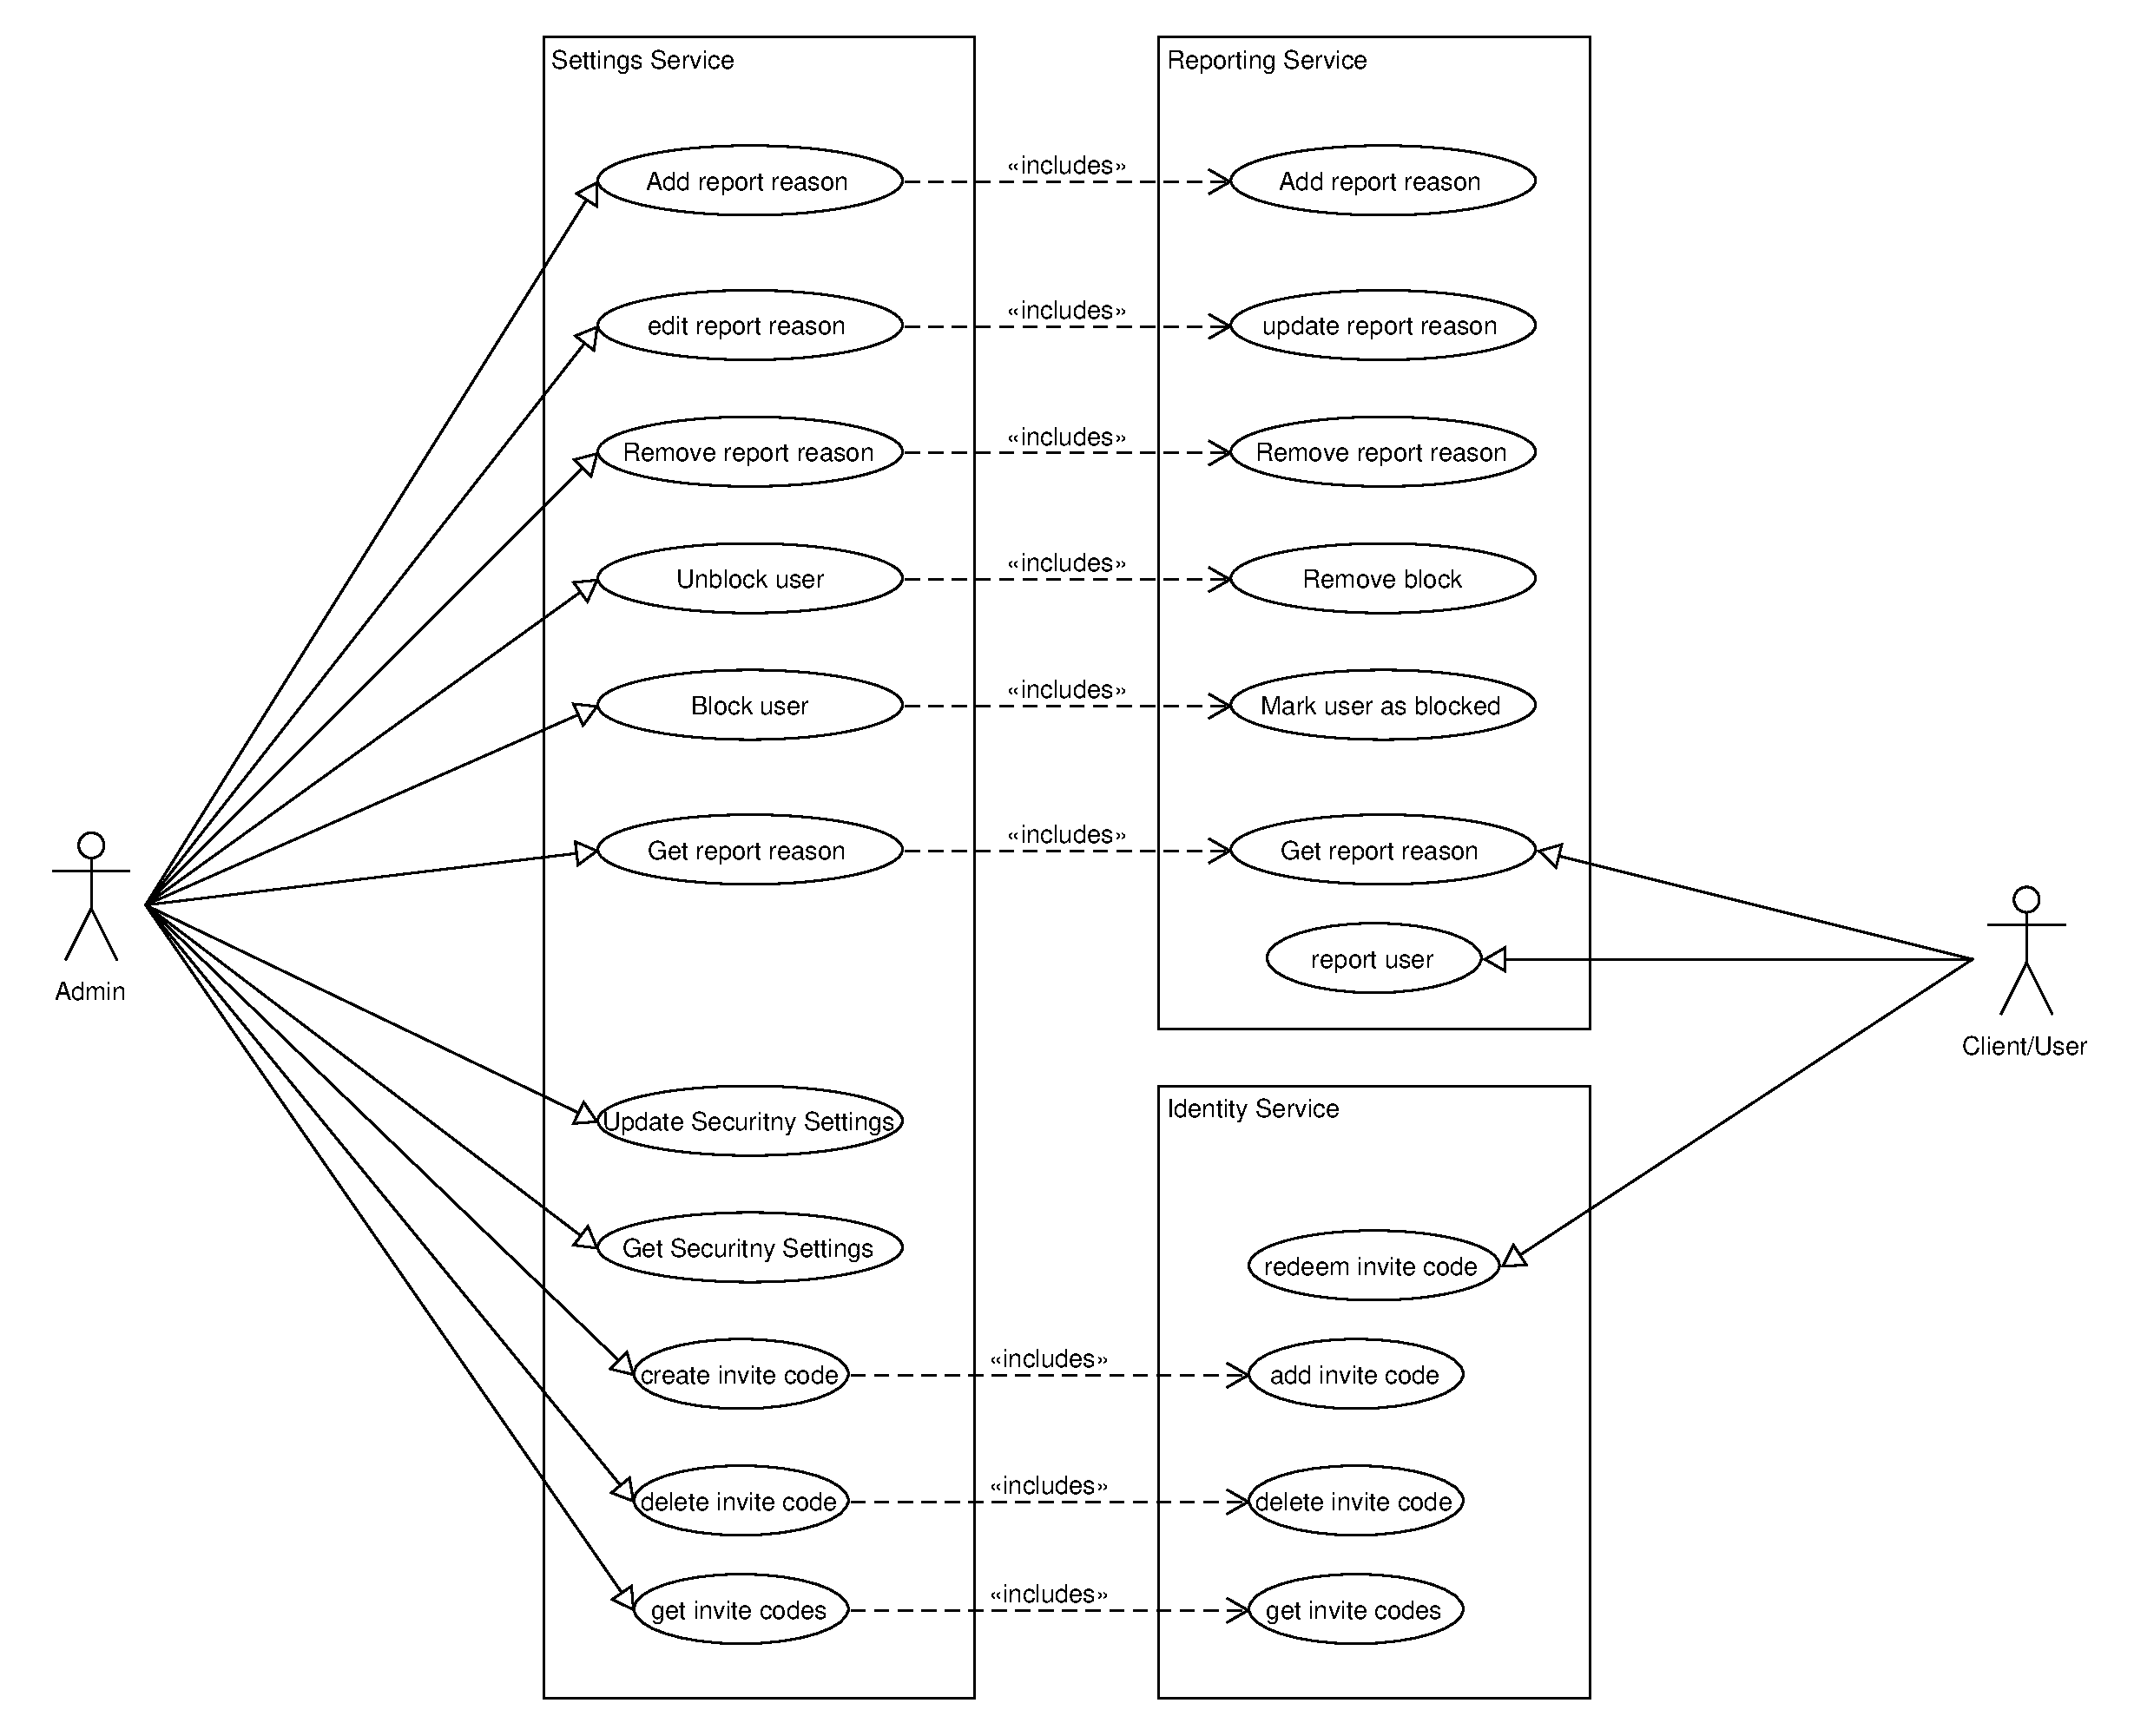
\includegraphics[width=1.0\textwidth]{./graphics/UseCaseDiagramAdminPanel}
    \caption{Use case diagram for admin panel}
    \label{fig:figure5}
\end{figure}

\subsection{Constraints}
% TODO which constraints exist for the project… find more

This Subsection provides a general description of some of the limitations of the chat application which should be taken
into consideration by developers.
Currently the system has limitations on the following areas:

\paragraph{Control Functions}
The system should contain certain access control functionality.
This means normal users should not be able to conduct administrative tasks, whilst admin users should not be able to
access the chat system itself but only conduct administrative tasks.

\paragraph{Safety and Security Considerations}
The chat service should be fully end-to-end encrypted and secure from third parties.

\paragraph{Registration}
If the Administrators have set that invite codes are mandatory to register to the web service, users without an invite
could should not be able to gain access into the chat application.

\paragraph{Banned Users}
If an admin decides to ban a user, the user should not have the possibility to get access to the application.
All data locally stored on the user’s device should be deleted after the first try of login, after the user was banned.
This guarantees that no banned user is in the possession of private chat data.

\paragraph{Received Receipts}
Received receipts are only send if the receiver set to show them.

\paragraph{Read Receipts}
Read receipts are only send if the receiver set to show them.


\section{Specific Requirements}\label{sec:specific-requirements}
This section of the SRS will contain all of functional and quality requirements and will also give a detailed
description of what features the system will have.

\subsection{External Interface Requirements}\label{subsec:external-interface-requirements}
This section provides a detailed description of all inputs and outputs from the elevator system and gives a description
of software and communication interfaces.

\paragraph{User Interfaces}
\begin{itemize}
    \item The user Interface will consist of a chat application.
    Here the user will be able to log in to/ out of the application.
    Once logged in, the user will be able to see all his contacts, add new contacts, send chat/voice messages to their
    contacts, send files to their contacts, view contact details, report contacts.
    % TODO frontend team: check if every UI feature has been mentioned here
    \item The admin interface/admin panel will allow the admin user to conduct administrative settings for the server.
    This will include general server settings, like duo authentication, password requirements for users, whether users
    require an invitation in the first place to join the server, etc.
    Furthermore, the admin can handle the reporting system here, meaning they will be able to add and remover reasons
    for which a normal user can be reported for.
    It will provide a list with an anonymous overview of all users that are currently reported and or blocked.
    Users will be able to be unblocked via the admin panel.
    Lastly the panel will contain a dashboard with some information of the server (e.g.\ traffic, amounts of reports in
    the past etc.)
\end{itemize}

\paragraph{Software Interfaces}
% TODO Jörn Neumeyer: maybe say a few words to the encryption protocol, what it could be used for in the future, etc. (?)

\subsection{Functional and Performance Requirements}\label{subsec:functional-and-performance-requirements}

This section includes the requirements that specify all fundamental actions of the software system and performance
requirements the software system should consider.
This part of the document will describe the use cases of the different user groups of the system.

\begin{table}[ht]
    \centering
    \caption{Register}
    \begin{tabular}{|L{5cm}|L{10cm}|}
        \toprule
        \textbf{Name}         & Register                                    \\
        \textbf{Actor}        & User                                        \\
        \textbf{Description}  & Actor registers at a server                 \\
        \textbf{Precondition} & N/A                                         \\
        \textbf{Scenario} &
        \vspace{-0.75cm}
        \begin{enumerate}
            \setlength\itemsep{-0.5em}
            \item The actor enters the login page
            \item The actor chooses to register a new account
            \item The system directs the actor to the registration form
            \item The actor enters the server details as well as their username and password
            \item The actor chooses to confirm their details
            \item The system registers the user
        \end{enumerate} \\[-0.5cm]
        \textbf{Result}       & The actor has been registered in the system \\
        \textbf{Exceptions}   & N/A                                         \\
        \bottomrule
    \end{tabular}
    \label{tab:table7}
\end{table}

\begin{table}[ht]
    \caption{Login}
    \begin{tabular}{|L{5cm}|L{10cm}|}
        \toprule
        \textbf{Name}         & Login                                                                              \\
        \textbf{Actor}        & User                                                                               \\
        \textbf{Description}  & The actor logs in to the system                                                    \\
        \textbf{Precondition} & The actor has to be \textbf{\hyperref[tab:table7]{registered}}                     \\
        \textbf{Scenario} &
        \vspace{-0.75cm}
        \begin{enumerate}
            \setlength\itemsep{-0.5em}
            \item The actor navigates to the login
            \item The actor provides their login credentials, and the server details
            \item The system verifies the login credentials
            \item The system logs in the actor
        \end{enumerate} \\[-0.5cm]
        \textbf{Result}       & The actor is logged in                                                             \\
        \textbf{Exceptions}   & if credentials are invalid: the system notifies the actor about invalid credential \\
        \bottomrule
    \end{tabular}
    \label{tab:table8}
\end{table}

\begin{table}[ht]
    \caption{Send message}
    \begin{tabular}{|L{5cm}|L{10cm}|}
        \toprule
        \textbf{Name}        & Send message                              \\
        \textbf{Actor}       & User                                      \\
        \textbf{Description} & The actor sends a message to another user \\
        \textbf{Precondition} &
        \vspace{-0.75cm}
        \begin{itemize}
            \setlength\itemsep{-0.5em}
            \item The actor has to be \textbf{\hyperref[tab:table8]{logged in}}
            \item The actor to send the message to has to be in the actors contact list
        \end{itemize} \\[-0.5cm]
        \textbf{Scenario} &
        \vspace{-0.75cm}
        \begin{enumerate}
            \setlength\itemsep{-0.5em}
            \item The actor chooses a user to send a message to
            \item The system navigates to the chat of the selected user
            \item The actor enters the message and chooses to send it
            \item The system sends the message to the chat partner
        \end{enumerate} \\[-0.5cm]
        \textbf{Result}      & The message has been sent                 \\
        \textbf{Exceptions}  & N/A                                       \\
        \bottomrule
    \end{tabular}
    \label{tab:table9}
\end{table}

\begin{table}[ht]
    \caption{Logout}
    \begin{tabular}{|L{5cm}|L{10cm}|}
        \toprule
        \textbf{Name}         & Logout                                                        \\
        \textbf{Actor}        & User                                                          \\
        \textbf{Description}  & The actor chooses to log out of the system                    \\
        \textbf{Precondition} & The actor has to be \textbf{\hyperref[tab:table8]{logged in}} \\
        \textbf{Scenario} &
        \vspace{-0.75cm}
        \begin{enumerate}
            \setlength\itemsep{-0.5em}
            \item The actor navigates to the login
            \item The actor provides their login credentials, and the server details
            \item The system verifies the login credentials
            \item The system logs in the actor
        \end{enumerate} \\[-0.5cm]
        \textbf{Result}       & The actor is logged out                                       \\
        \textbf{Exceptions}   & N/A                                                           \\
        \bottomrule
    \end{tabular}
    \label{tab:table10}
\end{table}

\begin{table}[ht]
    \caption{Search User}
    \begin{tabular}{|L{5cm}|L{10cm}|}
        \toprule
        \textbf{Name}         & Search User                                                   \\
        \textbf{Actor}        & User                                                          \\
        \textbf{Description}  & The actor searches for a user to continue a chat with         \\
        \textbf{Precondition} & The actor has to be \textbf{\hyperref[tab:table8]{logged in}} \\
        \textbf{Scenario} &
        \vspace{-0.75cm}
        \begin{enumerate}
            \setlength\itemsep{-0.5em}
            \item The actor enters a username
            \item The system displays the matching chat partners
            \item The actor selects a user to start a chat
        \end{enumerate} \\[-0.5cm]
        \textbf{Result}       & The actor selected a chat partner                             \\
        \textbf{Exceptions} & 3a.
        The system can not find a chat partner for the provided username.
        System: "no user found" \\
        \bottomrule
    \end{tabular}
    \label{tab:table11}
\end{table}

\begin{table}[ht]
    \caption{Block user}
    \begin{tabular}{|L{5cm}|L{10cm}|}
        \toprule
        \textbf{Name}         & Block user                                                          \\
        \textbf{Actor}        & User                                                                \\
        \textbf{Description}  & An actor blocks another user to prevent receiving messages of them  \\
        \textbf{Precondition} & The actor has to be \textbf{\hyperref[tab:table8]{logged in}}       \\
        \textbf{Scenario} &
        \vspace{-0.75cm}
        \begin{enumerate}
            \setlength\itemsep{-0.5em}
            \item The actor chooses a user to block
            \item The system navigates to the chat of the selected chat partner
            \item The actor chooses to **view the profile** of the user %TODO add reference
            \item The system shows the profile of the selected user
            \item The actor chooses to block the user
            \item The system acknowledges the decision
        \end{enumerate} \\[-0.5cm]
        \textbf{Result}       & The selected user is not able to send messages to the actor anymore \\
        \textbf{Exceptions}   & N/A                                                                 \\
        \bottomrule
    \end{tabular}
    \label{tab:table12}
\end{table}

\begin{table}[ht]
    \caption{Change Settings}
    \begin{tabular}{|L{5cm}|L{10cm}|}
        \toprule
        \textbf{Name}         & Change Settings                                               \\
        \textbf{Actor}        & User                                                          \\
        \textbf{Description}  & Actor changes settings                                        \\
        \textbf{Precondition} & The actor has to be \textbf{\hyperref[tab:table8]{logged in}} \\
        \textbf{Scenario} &
        \vspace{-0.75cm}
        \begin{enumerate}
            \setlength\itemsep{-0.5em}
            \item Actor selects the hamburger menu button
            \item System displays options to interact with
            \item Actor selects settings
            \item System displays settings
            \item Actor selects setting to change
            \item System displays a confirmation message
            \item Actor selects confirm changes
            \item System changed settings
        \end{enumerate} \\[-0.5cm]
        \textbf{Result}       & Actor has changed the settings                                \\
        \textbf{Exceptions} & 5.
        Actor is not authorized to change this setting \\
        \textbf{Alternate Flow} & 7a.
        Actor selects cancel changes \\
        \bottomrule
    \end{tabular}
    \label{tab:table13}
\end{table}

\begin{table}[ht]
    \caption{Set profile picture}
    \begin{tabular}{|L{5cm}|L{10cm}|}
        \toprule
        \textbf{Name}         & Set profile picture                                                                            \\
        \textbf{Actor}        & User                                                                                           \\
        \textbf{Description}  & The actor can set their own profile picture, so it will be visible for their contacts later on \\
        \textbf{Precondition} & The actor has to be \textbf{\hyperref[tab:table8]{logged in}}                                  \\
        \textbf{Scenario} &
        \vspace{-0.75cm}
        \begin{enumerate}
            \setlength\itemsep{-0.5em}
            \item The actor navigates to settings
            \item The system shows the settings menu
            \item The actor navigates to profile settings
            \item The system shows the profile settings menu
            \item The actor selects \enquote{change profile picture}
            \item The actor selects and saves a picture
        \end{enumerate} \\[-0.5cm]
        \textbf{Result}       & The profile picture has been changed to the selected image                                     \\
        \textbf{Exceptions} & 4.
        The image file is in an unsupported file format \\
        \bottomrule
    \end{tabular}
    \label{tab:table14}
\end{table}

\begin{table}[ht]
    \caption{View profile picture}
    \begin{tabular}{|L{5cm}|L{10cm}|}
        \toprule
        \textbf{Name}         & View profile picture                                          \\
        \textbf{Actor}        & User                                                          \\
        \textbf{Description}  & The actor can view their profile picture                      \\
        \textbf{Precondition} & The actor has to be \textbf{\hyperref[tab:table8]{logged in}} \\
        \textbf{Scenario} &
        \vspace{-0.75cm}
        \begin{enumerate}
            \setlength\itemsep{-0.5em}
            \item The actor navigates to settings
            \item The system shows the settings menu
            \item The actor navigates to profile settings
            \item The system shows the profile settings menu
            \item The actor selects \enquote{view profile picture}
            \item The system shows the profile picture
        \end{enumerate} \\[-0.5cm]
        \textbf{Result}       & The profile picture is displayed to the user                  \\
        \textbf{Exceptions} & 6.
        If the user does not have a profile picture a placeholder image should be shown \\
        \bottomrule
    \end{tabular}
    \label{tab:table15}
\end{table}

\begin{table}[ht]
    \caption{Open chat}
    \begin{tabular}{|L{5cm}|L{10cm}|}
        \toprule
        \textbf{Name}        & Open chat                 \\
        \textbf{Actor}       & User                      \\
        \textbf{Description} & Actor opens a chat        \\
        \textbf{Precondition} &
        \vspace{-0.75cm}
        \begin{itemize}
            \setlength\itemsep{-0.5em}
            \item The actor has to be \textbf{\hyperref[tab:table8]{logged in}}
            \item Actor has chats available
        \end{itemize} \\[-0.5cm]
        \textbf{Scenario} &
        \vspace{-0.75cm}
        \begin{enumerate}
            \setlength\itemsep{-0.5em}
            \item Actor selects a chat in the list of recently opened chats
            \item System displays the chat and corresponding chat history
        \end{enumerate} \\[-0.5cm]
        \textbf{Result}      & Actor has opened the chat \\
        \textbf{Exceptions}  & N/A                       \\
        \bottomrule
    \end{tabular}
    \label{tab:table16}
\end{table}

\begin{table}[ht]
    \caption{Start new chat}
    \begin{tabular}{|L{5cm}|L{10cm}|}
        \toprule
        \textbf{Name}        & Start new chat               \\
        \textbf{Actor}       & User                         \\
        \textbf{Description} & Actor starts a new chat      \\
        \textbf{Precondition} &
        \vspace{-0.75cm}
        \begin{itemize}
            \setlength\itemsep{-0.5em}
            \item The actor has to be \textbf{\hyperref[tab:table8]{logged in}}
            \item Actor has **searched** for a user % TODO add reference to search
        \end{itemize} \\[-0.5cm]
        \textbf{Scenario} &
        \vspace{-0.75cm}
        \begin{enumerate}
            \setlength\itemsep{-0.5em}
            \item Actor selects a contact person to start the chat with in the search result list
            \item System displays the chat
        \end{enumerate} \\[-0.5cm]
        \textbf{Result}      & Actor has started a new chat \\
        \textbf{Exceptions} & 2.
        Selected user has blocked the actor.
        The system will reject to start a new chat. \\
        \bottomrule
    \end{tabular}
    \label{tab:table17}
\end{table}

\begin{table}[ht]
    \caption{Send voice message}
    \begin{tabular}{|L{5cm}|L{10cm}|}
        \toprule
        \textbf{Name}        & Send voice message                                         \\
        \textbf{Actor}       & User                                                       \\
        \textbf{Description} & An actor records a message and sends it to another user    \\
        \textbf{Precondition} &
        \vspace{-0.75cm}
        \begin{itemize}
            \setlength\itemsep{-0.5em}
            \item The actor has to be \textbf{\hyperref[tab:table8]{logged in}}
            \item Actor has a chat partner selected
        \end{itemize} \\[-0.5cm]
        \textbf{Scenario} &
        \vspace{-0.75cm}
        \begin{enumerate}
            \setlength\itemsep{-0.5em}
            \item The actor chooses to send a voice message
            \item The system starts to record the actors voice
            \item The actor choose to send the voice message
            \item The system stops recording
            \item The system sends the recorded message
        \end{enumerate} \\[-0.5cm]
        \textbf{Extensions} & 3a.
        The actor chooses to cancel the recording.
        The System stops recording. \\
        \textbf{Result}      & The voice message of the actor is sent to the chat partner \\
        \textbf{Exceptions}  & N/A                                                        \\
        \bottomrule
    \end{tabular}
    \label{tab:table18}
\end{table}

\begin{table}[ht]
    \caption{Send file}
    \begin{tabular}{|L{5cm}|L{10cm}|}
        \toprule
        \textbf{Name}        & Send file                                           \\
        \textbf{Actor}       & User                                                \\
        \textbf{Description} & An actor selects a file and send it to another user \\
        \textbf{Precondition} &
        \vspace{-0.75cm}
        \begin{itemize}
            \setlength\itemsep{-0.5em}
            \item The actor has to be \textbf{\hyperref[tab:table8]{logged in}}
            \item Actor has a chat partner selected
        \end{itemize} \\[-0.5cm]
        \textbf{Scenario} &
        \vspace{-0.75cm}
        \begin{enumerate}
            \setlength\itemsep{-0.5em}
            \item The actor chooses to send a file
            \item The system shows a file explorer
            \item The actor selects a file to send
            \item The system sends the file to the chat partner
        \end{enumerate} \\[-0.5cm]
        \textbf{Extensions} & 2a.
        The actor chooses multiple files.
        The System sends the files to the chat partner. \\
        \textbf{Result}      & The file is sent to the chat partner                \\
        \textbf{Exceptions}  & N/A                                                 \\
        \bottomrule
    \end{tabular}
    \label{tab:table19}
\end{table}

\begin{table}[ht]
    \caption{Delete message}
    \begin{tabular}{|L{5cm}|L{10cm}|}
        \toprule
        \textbf{Name}        & Delete message                                     \\
        \textbf{Actor}       & User                                               \\
        \textbf{Description} & The actor can delete a message from a conversation \\
        \textbf{Precondition} &
        \vspace{-0.75cm}
        \begin{itemize}
            \setlength\itemsep{-0.5em}
            \item The actor has to be \textbf{\hyperref[tab:table8]{logged in}}
            \item Actor has a chat partner selected
            \item There must be at least one message which can be deleted
        \end{itemize} \\[-0.5cm]
        \textbf{Scenario} &
        \vspace{-0.75cm}
        \begin{enumerate}
            \setlength\itemsep{-0.5em}
            \item The actor selects a message in the opened chat
            \item The system displays options to interact with the highlighted message
            \item The actor decides to delete the message from the conversation
            \item The system removes the message from the conversation
        \end{enumerate} \\[-0.5cm]
        \textbf{Result}      & The selected message is deleted                    \\
        \textbf{Exceptions}  & N/A                                                \\
        \bottomrule
    \end{tabular}
    \label{tab:table20}
\end{table}

\begin{table}[ht]
    \caption{Delete conversation}
    \begin{tabular}{|L{5cm}|L{10cm}|}
        \toprule
        \textbf{Name}        & Delete message                               \\
        \textbf{Actor}       & User                                         \\
        \textbf{Description} & The actor can delete a complete conversation \\
        \textbf{Precondition} &
        \vspace{-0.75cm}
        \begin{itemize}
            \setlength\itemsep{-0.5em}
            \item The actor has to be \textbf{\hyperref[tab:table8]{logged in}}
            \item There must be at least one conversation which can be deleted
        \end{itemize} \\[-0.5cm]
        \textbf{Scenario} &
        \vspace{-0.75cm}
        \begin{enumerate}
            \setlength\itemsep{-0.5em}
            \item The actor selects a conversation from the conversation overview
            \item The system displays options to interact with the highlighted conversation
            \item The actor decides to delete the conversation from the conversation overview
            \item The system removes the conversation
        \end{enumerate} \\[-0.5cm]
        \textbf{Result}      & The selected conversation is deleted         \\
        \textbf{Exceptions}  & N/A                                          \\
        \bottomrule
    \end{tabular}
    \label{tab:table21}
\end{table}

\begin{table}[ht]
    \caption{Star message}
    \begin{tabular}{|L{5cm}|L{10cm}|}
        \toprule
        \textbf{Name}        & Star message                \\
        \textbf{Actor}       & User                        \\
        \textbf{Description} & Actor stars a message       \\
        \textbf{Precondition} &
        \vspace{-0.75cm}
        \begin{itemize}
            \setlength\itemsep{-0.5em}
            \item The actor has to be \textbf{\hyperref[tab:table8]{logged in}}
            \item Actor has opened a chat
            \item Message is available
        \end{itemize} \\[-0.5cm]
        \textbf{Scenario} &
        \vspace{-0.75cm}
        \begin{enumerate}
            \setlength\itemsep{-0.5em}
            \item Actor selects a message in the opened chat
            \item System displays options to interact with the highlighted message
            \item Actor selects the star button
            \item System displays that the message is now starred
        \end{enumerate} \\[-0.5cm]
        \textbf{Result}      & Actor has starred a message \\
        \textbf{Exceptions}  & N/A                         \\
        \bottomrule
    \end{tabular}
    \label{tab:table22}
\end{table}

\begin{table}[ht]
    \caption{Change settings}
    \begin{tabular}{|L{5cm}|L{10cm}|}
        \toprule
        \textbf{Name}         & Change settings                                                   \\
        \textbf{Actor}        & Admin                                                             \\
        \textbf{Description}  & This use case describes the act of changing the security settings \\
        \textbf{Precondition} & N/A                                                               \\
        \textbf{Scenario} &
        \vspace{-0.75cm}
        \begin{enumerate}
            \setlength\itemsep{-0.5em}
            \item The actor presents the new security settings
            \item The system verifies the security settings
            \item The system enters the new security settings
            \item The system notifies the actor about the successful insertion of the settings
        \end{enumerate} \\[-0.5cm]
        \textbf{Result}       & The security settings have been updated                           \\
        \textbf{Exceptions} &
        \vspace{-0.75cm}
        \begin{itemize}
            \setlength\itemsep{-0.5em}
            \item The settings contain an invalid attribute
            \item The system notifies the user about the wrong attribute
        \end{itemize} \\
        \bottomrule
    \end{tabular}\label{tab:table25}
\end{table}

\begin{table}[ht]
    \caption{Create report reason}
    \begin{tabular}{|L{5cm}|L{10cm}|}
        \toprule
        \textbf{Name}         & Create report reason                                              \\
        \textbf{Actor}        & Admin                                                             \\
        \textbf{Description}  & This use case describes the procedure of creating a report reason \\
        \textbf{Precondition} & N/A                                                               \\
        \textbf{Scenario} &
        \vspace{-0.75cm}
        \begin{enumerate}
            \setlength\itemsep{-0.5em}
            \item The system receives a report reason
            \item The system validates the report reason
            \item The system adds the report reason
            \item The system notifies the client that the reason has been added
        \end{enumerate} \\[-0.5cm]
        \textbf{Result}       & A report reason has been added                                    \\
        \textbf{Exceptions} &
        \vspace{-0.75cm}
        \begin{itemize}
            \setlength\itemsep{-0.5em}
            \item The reason contains invalid attributes
            \item The system notifies the client about the invalid attributes
        \end{itemize} \\
        \bottomrule
    \end{tabular}
    \label{tab:table26}
\end{table}

\begin{table}[ht]
    \caption{Ban user}
    \begin{tabular}{|L{5cm}|L{10cm}|}
        \toprule
        \textbf{Name}         & Ban user                                                                                        \\
        \textbf{Actor}        & Admin                                                                                           \\
        \textbf{Description}  & This use case describes the procedure of banning a user/removing their access to the system     \\
        \textbf{Precondition} & Actor is logged in                                                                              \\
        \textbf{Scenario} &
        \vspace{-0.75cm}
        \begin{enumerate}
            \setlength\itemsep{-0.5em}
            \item Actor views user and decides to block a user
            \item System \hyperref[tab:table28]{\textbf{blocks the user}}
            \item System applies the login ban and informs the actor about the result
        \end{enumerate} \\[-0.5cm]
        \textbf{Result}       & The user to ban can not login into the system anymore and all current logins will be terminated \\
        \textbf{Exceptions} &
        \vspace{-0.75cm}
        \begin{itemize}
            \setlength\itemsep{-0.5em}
            \item 1. System message: \enquote{unknown user}
            \item 1.1 Use case ends here
        \end{itemize} \\
        \bottomrule
    \end{tabular}
    \label{tab:table27}
\end{table}

\begin{table}[ht]
    \caption{Block user}
    \begin{tabular}{|L{5cm}|L{10cm}|}
        \toprule
        \textbf{Name}         & Block user                                                                                       \\
        \textbf{Actor}        & Admin                                                                                            \\
        \textbf{Description}  & This use case describes the procedure of banning a user/removing their access to the system      \\
        \textbf{Precondition} & Actor is logged in                                                                               \\
        \textbf{Scenario} &
        \vspace{-0.75cm}
        \begin{enumerate}
            \setlength\itemsep{-0.5em}
            \item The system receives the task to block a user
            \item The system marks a user as marked
            \item The system notifies the client that the block has been executed
        \end{enumerate} \\[-0.5cm]
        \textbf{Result}       & The user to ban can not log in into the system anymore and all current logins will be terminated \\
        \textbf{Exceptions} &
        \vspace{-0.75cm}
        \begin{itemize}
            \setlength\itemsep{-0.5em}
            \item 1. System message: \enquote{unknown user}
            \item 1.1 Use case ends here
        \end{itemize} \\
        \bottomrule
    \end{tabular}
    \label{tab:table28}
\end{table}

\begin{table}[ht]
    \caption{Login}
    \begin{tabular}{|L{5cm}|L{10cm}|}
        \toprule
        \textbf{Name}         & Login                                                  \\
        \textbf{Actor}        & Admin                                                  \\
        \textbf{Description}  & The login process for the admin user                   \\
        \textbf{Precondition} & N/A                                                    \\
        \textbf{Scenario} &
        \vspace{-0.75cm}
        \begin{enumerate}
            \setlength\itemsep{-0.5em}
            \item Actor enters their credentials into the system
            \item System checks actor's credentials
            \item System informs actor about the login success
            \item Actor is logged into the system
        \end{enumerate} \\[-0.5cm]
        \textbf{Result}       & The actor has been successfully logged into the system \\
        \textbf{Exceptions} &
        \vspace{-0.75cm}
        \begin{itemize}
            \setlength\itemsep{-0.5em}
            \item 3. The actor's credentials were invalid.
            \item 3.1 Use case ends here.
        \end{itemize} \\
        \bottomrule
    \end{tabular}
    \label{tab:table28}
\end{table}

\begin{table}[ht]
    \caption{Edit report reason}
    \begin{tabular}{|L{5cm}|L{10cm}|}
        \toprule
        \textbf{Name}         & Edit report reason                                               \\
        \textbf{Actor}        & Admin                                                            \\
        \textbf{Description}  & This use case describes the procedure of editing a report reason \\
        \textbf{Precondition} & There must be at least one reason to be edited                   \\
        \textbf{Scenario} &
        \vspace{-0.75cm}
        \begin{enumerate}
            \setlength\itemsep{-0.5em}
            \item The user decides to edit a report reason
            \item The system updates a report reason
            \item The system notifies the client that the reason has been edited successfully
        \end{enumerate} \\[-0.5cm]
        \textbf{Result}       & A report reason has been edited                                  \\
        \textbf{Exceptions}   & N/A                                                              \\
        \bottomrule
    \end{tabular}
    \label{tab:table29}
\end{table}

\begin{table}[ht]
    \caption{Generate Invite}
    \begin{tabular}{|L{5cm}|L{10cm}|}
        \toprule
        \textbf{Name}        & Generate Invite                                                        \\
        \textbf{Actor}       & Admin                                                                  \\
        \textbf{Description} & The actor may generate invitation codes for new users to register with \\
        \textbf{Precondition} &
        \vspace{-0.75cm}
        \begin{enumerate}
            \setlength\itemsep{-0.5em}
            \item Actor is logged in
            \item System requires invitation codes for new users to register
        \end{enumerate} \\[-0.5cm] \\
        \textbf{Scenario} &
        \vspace{-0.75cm}
        \begin{enumerate}
            \setlength\itemsep{-0.5em}
            \item Actor opens an overview of system settings
            \item System shows the available settings of the system
            \item Actor navigates to registration invitations section
            \item System displays registration invitations options
            \item Actor triggers action \enquote{Generate Invitation Code}
            \item System generates an invitation code for user registration and displays it to the actor
        \end{enumerate} \\[-0.5cm]
        \textbf{Result}  & A new registration invitation/code was generated and persisted, so a user may use
        it for the registration process                                                                    \\
        \textbf{Exceptions}  & N/A                                                                    \\
        \bottomrule
    \end{tabular}
    \label{tab:table30}
\end{table}

\begin{table}[ht]
    \caption{Get all report reasons}
    \begin{tabular}{|L{5cm}|L{10cm}|}
        \toprule
        \textbf{Name}         & Get all report reasons                 \\
        \textbf{Actor}        & Admin                                  \\
        \textbf{Description}  & The actor gets all report reasons      \\
        \textbf{Precondition} & Actor is logged in                     \\
        \textbf{Scenario} &
        \vspace{-0.75cm}
        \begin{enumerate}
            \setlength\itemsep{-0.5em}
            \item The actor wishes to view all report reasons
            \item The system shows the actors all report reasons
        \end{enumerate} \\[-0.5cm]
        \textbf{Result}       & The system displays all report reasons \\
        \textbf{Exceptions}   & N/A                                    \\
        \bottomrule
    \end{tabular}
    \label{tab:table31}
\end{table}

\begin{table}[ht]
    \caption{Remove invite code}
    \begin{tabular}{|L{5cm}|L{10cm}|}
        \toprule
        \textbf{Name}         & Remove invite code                                             \\
        \textbf{Actor}        & Admin                                                          \\
        \textbf{Description}  & This use case describes the process of removing an invite code \\
        \textbf{Precondition} & Actor is logged in                                             \\
        \textbf{Scenario} &
        \vspace{-0.75cm}
        \begin{enumerate}
            \setlength\itemsep{-0.5em}
            \item The actor wishes to delete all report reasons
            \item The actor selects the invite code which is to be deleted
            \item The system deletes the invite code
            \item The system lets the actor know that the code has been deleted
        \end{enumerate} \\[-0.5cm]
        \textbf{Result}       & An invite code has been deleted                                \\
        \textbf{Exceptions}   & N/A                                                            \\
        \bottomrule
    \end{tabular}
    \label{tab:table32}
\end{table}

\begin{table}[ht]
    \caption{Delete report reason}
    \begin{tabular}{|L{5cm}|L{10cm}|}
        \toprule
        \textbf{Name}         & Delete report reason                                              \\
        \textbf{Actor}        & Admin                                                             \\
        \textbf{Description}  & This use case describes the procedure of deleting a report reason \\
        \textbf{Precondition} & Actor is logged in                                                \\
        \textbf{Scenario} &
        \vspace{-0.75cm}
        \begin{enumerate}
            \setlength\itemsep{-0.5em}
            \item The actor selects the reason to be deleted
            \item The system receives the reason which is to be deleted
            \item The system deletes the report reason
            \item The system notifies the client that the reason has been deleted
        \end{enumerate} \\[-0.5cm]
        \textbf{Result}       & A report reason has been deleted                                  \\
        \textbf{Exceptions}   & N/A                                                               \\
        \bottomrule
    \end{tabular}
    \label{tab:table33}
\end{table}

\begin{table}[ht]
    \caption{Require invite}
    \begin{tabular}{|L{5cm}|L{10cm}|}
        \toprule
        \textbf{Name}         & Require invite     \\
        \textbf{Actor}        & Admin              \\
        \textbf{Description} & In this use case, the actor changes the server settings, so invitation codes are
        required for user registrations or not. \\
        \textbf{Precondition} & Actor is logged in \\
        \textbf{Scenario} &
        \vspace{-0.75cm}
        \begin{enumerate}
            \setlength\itemsep{-0.5em}
            \item Actor opens an overview of system settings
            \item System shows the available settings of the system
            \item Actor changes the setting \enquote{Registration invitations} to \enquote{required} or \enquote{off}
            \item  System applies the requested settings change
        \end{enumerate} \\[-0.5cm]
        \textbf{Result} & If property is set to \enquote{required}, the system now requires invitation codes to
        be present on user registration. \\
        \textbf{Exceptions}   & N/A                \\
        \bottomrule
    \end{tabular}
    \label{tab:table34}
\end{table}

\begin{table}[ht]
    \caption{Require E-Mail confirmation }
    \begin{tabular}{|L{5cm}|L{10cm}|}
        \toprule
        \textbf{Name}         & Require E-Mail confirmation \\
        \textbf{Actor}        & Admin                       \\
        \textbf{Description} & In this use case, the actor changes the server settings, so E-Mail confirmation for user
        registration is required, or not. \\
        \textbf{Precondition} & Actor is logged in          \\
        \textbf{Scenario} &
        \vspace{-0.75cm}
        \begin{enumerate}
            \setlength\itemsep{-0.5em}
            \item Actor opens an overview of system settings
            \item System shows the available settings of the system
            \item Actor changes the setting \enquote{E-Mail Confirmation} to \enquote{required} or \enquote{off}
            \item  System applies the requested settings change
        \end{enumerate} \\[-0.5cm]
        \textbf{Result} & If property is set to \enquote{required}, the system now requires a valid e-mail address to be
        present on user registration as well as confirming the validity of said e-mail address. \\
        \textbf{Exceptions}   & N/A                         \\
        \bottomrule
    \end{tabular}
    \label{tab:table35}
\end{table}

\begin{table}[ht]
    \caption{Require E-2FA }
    \begin{tabular}{|L{5cm}|L{10cm}|}
        \toprule
        \textbf{Name}         & Require 2FA      \\
        \textbf{Actor}        & Admin              \\
        \textbf{Description} & In this use case, the actor changes the server settings, so two-factor authentication is
        required for users, or not.   \\
        \textbf{Precondition} & Actor is logged in \\
        \textbf{Scenario} &
        \vspace{-0.75cm}
        \begin{enumerate}
            \setlength\itemsep{-0.5em}
            \item Actor opens an overview of system settings
            \item System shows the available settings of the system
            \item Actor changes the setting \enquote{E-Two Factor Authentication} to \enquote{required} or \enquote{off}
            \item  System applies the requested settings change
        \end{enumerate} \\[-0.5cm]
        \textbf{Result} & If property is set to \enquote{required}, the system now requires two-factor authentication
        codes to be present on user registration and login. \\
        \textbf{Exceptions}   & N/A                \\
        \bottomrule
    \end{tabular}
    \label{tab:table36}
\end{table}

\begin{table}[ht]
    \caption{Add invite code}
    \begin{tabular}{|L{5cm}|L{10cm}|}
        \toprule
        \textbf{Name}         & Add invite code      \\
        \textbf{Actor}        & Admin              \\
        \textbf{Description} & This use case describes the procedure of creating an invite code \\
        \textbf{Precondition} & Actor is logged in \\
        \textbf{Scenario} &
        \vspace{-0.75cm}
        \begin{enumerate}
            \setlength\itemsep{-0.5em}
            \item Actor enters or selects to create an invite code
            \item The system receives an invite code
            \item The system validates the invite code
            \item The system adds the invite code
            \item The system notifies the client that the invite code has been added
        \end{enumerate} \\[-0.5cm]
        \textbf{Result} &  An invite code has been added \\
        \textbf{Exceptions}   & N/A                \\
        \bottomrule
    \end{tabular}
    \label{tab:table37}
\end{table}

\begin{table}[ht]
    \caption{Delete invite code}
    \begin{tabular}{|L{5cm}|L{10cm}|}
        \toprule
        \textbf{Name}         & Delete invite code      \\
        \textbf{Actor}        & Admin              \\
        \textbf{Description} & This use case describes the process of deleting an invite code  \\
        \textbf{Precondition} & Actor is logged in \\
        \textbf{Scenario} &
        \vspace{-0.75cm}
        \begin{enumerate}
            \setlength\itemsep{-0.5em}
            \item Actor selects the invite code to be deleted
            \item The system deletes the invite code
            \item The system lets the actor know that the code has been deleted
        \end{enumerate} \\[-0.5cm]
        \textbf{Result} &  An invite code has been deleted \\
        \textbf{Exceptions}   & N/A                \\
        \bottomrule
    \end{tabular}
    \label{tab:table38}
\end{table}
